%% ---------------------------------------------------------------------------
%% intro.tex
%%
%% Introduction
%%
%% $Id: intro.tex 1477 2010-07-28 21:34:43Z palvarado $
%% ---------------------------------------------------------------------------

\chapter{Introducción}
\label{chp:intro}
\section{Entorno de la tesis}

Costa Rica es uno de los países que se encuentran a la vanguardia en materia de conservación ambiental, esto debido al sistema de áreas protegidas, cerca del 25\% del territorio nacional cuenta con alguna categoría de protección. Las políticas nacionales de protección no sólo abogan por preservar la flora y fauna local sino también por mantener un desarrollo sostenible garantizando la perpetuidad de los recursos naturales. \cite{website:sinac}

Los recursos naturales son, innegablemente, el medio fundamental para el crecimiento integral de las sociedades modernas. Estos se encuentran implícitos en todas las actividades humanas y son indispensables para sostener el estilo de vida del ciudadano moderno, desde su nutrición, materia prima para la manufactura de la tecnología que emplea, los servicios que recibe, entre otros. \cite{website:inbio}

Por otra parte la riqueza natural representa una gran fuente de ingresos económicos para el país, debido al turismo. Según el informe del ICT, durante el primer trimestre del 2015 al país arribaron por todas las vías de ingreso un total de 811,379 personas, para el primer trimestre del 2016 arribaron un total de 919,624 lo que representa un incremento del 13.3\%. \cite{website:ict}

No obstante al marco jurídico en materia ambiental y los programas de protección ambiental hacia la flora y fauna, Costa Rica tiene serios problemas de caza furtiva y tala indiscriminada, pues los programas de conservación y la legislación actual son insuficientes para velar por la correcta protección de los recursos naturales (i.e. flora, fauna, minerales, etc), en mayor medida debido a la carencia de los fondos y personal necesarios para ejercer con más rigurosidad las políticas de conservación y penalización. De forma ilustrativa según el Sistema Nacional de Áreas de Conservación, en el 2014 eran necesarios, aproximadamente, 300 funcionarios dedicados al control y protección de las áreas protegidas (i.e. guardabosques) y el Estado era incapaz de hacer las contrataciones por falta de presupuesto. \cite{website:sinac}

Dado el dilema expuesto, estatalmente, se han puesto en marcha diversas estrategias para enfrentar la problemática; sin embargo, aumentar el recurso humano no es la opción más rentable para el Estado, siendo probable que una densidad mayor de guardabosques tampoco sea la solución. Partiendo de estas premisas se ha optado por un cambio de visión en camino a resolver el problema. Se considera que la posible solución resida en el uso de tecnología para facilitar la labor de los guardabosques.

Esta propuesta de solución tecnológica consiste en la implementación de una \textit{RIS} \footnote{\textit{RIS}: Acrónimo en español para Red Inalámbrica de Sensores} para vigilar de forma remota las zonas protegidas. Una \textit{RIS} no es otra cosa que una serie de dispositivos autónomos distribuidos en un área de interés, utilizando elementos de instrumentación (i.e. sensores) para monitorear condiciones físicas o ambientales. Cada miembro de la red corresponde a un nodo \cite{website:ni}. Se considera que si la \textit{RIS} no es la solución más viable, es una solución muy eficiente ya que las \textit{RIS} son capaces de medir parámetros, almacenarlos, procesarlos y enviarlos entre sí, lo cual permite ejecutar muchas de las labores realizables por un guardabosques. Como consideración especial, debe tenerse en cuenta que en un bosque no hay un acceso fácil a fuentes de alimentación eléctrica, por lo que es imperativo que la \textit{RIS} tenga un bajo consumo energético.

En respuesta a esta restricción, se presenta el proyecto: "Sonidos Ilegales" \cite{website:dcilab} de la Escuela de Ingeniería Electrónica del \textit{ITCR} \footnote{Instituto Tecnológico de Costa Rica} el cual refiere a la implementación de un sistema de reconocimiento de sonidos de motosierras, disparos de armas de fuego, como indicadores indirectos de actividades de tala y caza ilegales en zonas protegidas. Este proyecto consiste en el diseño de un sistema de hardware \textit{SoC} \footnote{SoC: Single on Chip. Sistema integrado en un chip} de bajo consumo energético el cual lleva a cabo las operaciones de procesamientos mencionas de la \textit{RIS}. \cite{website:inv_esc_electro, sirpa_SoC} 

El funcionamiento de una \textit{RIS} consiste en la obtención de muestras de señales
acústicas del medio, que en este caso se trata de un bosque. Seguidamente, los datos son iprocesados aplicando reconocimiento de patrones. En caso de encontrar un estado de alarma: disparo o motosierra, se activara el bloque de transmisión de información donde posteriormente la persona a cargo de la protección de la zona (el guardabosques), recibirá una notificación donde se le indicará el tipo de suceso y en cual nodo de la red se hizo de detección. En la figura \ref{nodoRIS} se muestra un diagrama de bloques de un nodo de la RIS que permite, a groso modo, entender el funcionamiento de la misma. \nocite{Carlosthesis}

\begin{figure}[h]
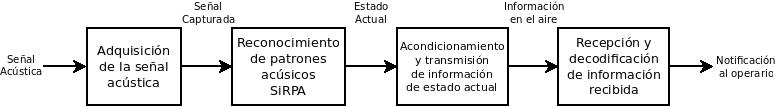
\includegraphics[width=\textwidth]{Nodo_RIS.jpeg}
\centering
\caption{Procesamiento realizado por cada nodo miembro de la RIS \cite{Jordanthesis}}
\label{nodoRIS}
\end{figure}


Interiorizando en la unidad de procesamiento, específicamente en el bloque denominado \textit{SiRPA} \footnote{SiRPA, es el acrónimo en español para Sistema de Reconocimiento de Patrones Acústicos}, este sigue una estructura estándar de un sistema de reconocimiento de patrones, el cual se compone de un bloque de preprocesado, una etapa de identificación/extracción de características fundamentales y un bloque de clasificación.

El preproceso consiste en acondicionar la señal analógica, en síntesis se refiere a normalizar y digitalizar la señal acústica. El bloque de identificación está compuesto por una batería de filtros, un estimador de energía, un reductor de dimensiones y un árbol clasificador. En el banco de filtros el espectro de la señal acústica se separa en 8 bandas distintas y luego se estima la energía a cada banda.

Mediante una transformación lineal, el reductor de dimensiones proyecta la salida del estimador de energía, que se encuentra en un espacio de ocho dimensiones, a un espacio de tres dimensiones. Según lo predice la \textit{maldición de dimensionalidad}, el conjunto de símbolos necesarios para describir de manera adecuada las observaciones realizadas es tres órdenes de magnitud superior si se emplea un espacio de ocho dimensiones en comparación a uno de tres. También tiene relación respecto a. \cite{NeuralNetworks, Jordanthesis}

El árbol binario o generador de símbolos, permite ubicar el centroide mas cercano a un patrón de entrada de tres dimensiones, para ello se utiliza la distancia L1 o Manhattan. Consecuentemente, los símbolos discretos se generan asociando estos, a las trayectorias continuas en el espacio del vector tridimensional de entrada, que describe la señal acústica en un determinado instante. El árbol binario genera un alfabeto de 32 símbolos discretos. \cite{IEEE_Panama, TDS, Jcardenas, EmbededTech}

Por último, encontramos la etapa de clasificación, encargada de calcular la probabilidad de que un conjunto de símbolos de entrada, formen parte de una señal acústica, de acuerdo con las categorías: bosque, motosierra o disparo. En este bloque, se utiliza un clasificador basado en la técnica de modelos ocultos de Markov (HMM). En la figura \ref{sirpa} se muestra un diagrama de bloques ilustrando como funciona internamente el SiRPA.

\begin{figure}[h]
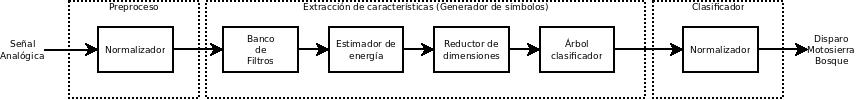
\includegraphics[width=\textwidth]{SiRPA.jpeg}
\centering
\caption{Diagrama de bloques del Sistema de Reconocimiento de Patrones Acústicos \cite{Carlosthesis}}
\label{sirpa}
\end{figure}


\section{Descripción del problema y justificación}

Como fue mencionado en el apartado anterior, países como Costa Rica ven amenazados sus recursos naturales por actividades ilegales como la caza furtiva y la tala. La tutela de los recursos naturales por parte del Estado es difícil, los bosques y los grandes mamíferos ven amenazada su conservación. En respuesta a esta situación la escuela de Ingeniería Electrónica del Instituto Tecnológico de Costa Rica, a través del \textit{DCILab} \footnote{DCILab: Laboratorio de Diseño de Circuitos Integrados} plantea una solución mediante un dispositivo electrónico de bajo consumo energético, capaz de reconocer sonidos como disparos de armas de fuego y motosierras. Esta iniciativa da a luz al proyecto SiRPA el cual pretende fabricar un \textit{ASIC} \footnote{ASIC es el acrónimo en inglés para: Circuito Integrado de Aplicación Especial... Se invita al lector a consultar un diccionario de términos electrónicos diccionario de términos electrónicos} con el fin de detectar la tala y caza ilegal en bosques, mediante el procesamiento digital de señales acústicas.

Luego de muchas etapas iterativas en el diseño del \textit{SiRPA}, el proyecto se encuentra codificado en un lenguaje de descripción de hardware (\textit{HDL}). Se han efectuado pruebas usando plataformas de sistemas embebidos como \textit{Beagle Boards} y textit{FPGAs} \footnotetext{Una FPGA (del inglés Field Programmable Gate Array) es un dispositivo electrónico que contiene bloques de lógica y electrónica digital que puede ser reconfigurada “in situ” mediante un lenguaje de descripción de hardware.} para la validación del diseño, se han publicado algunos papers al respecto, y se ha demostrado la viabilidad del proyecto, por lo que compete continuar la labor de
implementar la codificación \textit{HDL} a su etapa final, la cual consiste en la síntesis de los módulos
descritos en HDL sobre un chip de silicio.

Durante el 2014 el \textit{DCILab} contó con el apoyo del ingeniero argentino Dr. Juan Agustín Rodríguez, quien desarrolló un flujo de diseño digital sobre las herramientas de software Synopsys que implementan los módulos en HDL del \textit{SiRPA} al silicio para el circuito integrado. El trabajo del Dr.Rodríguez quedó incompleto y el \textit{SiRPA} no ha podido ser fabricado. Es por ello que el \textit{DCILab} requiere terminar el trabajo empezado por el Dr. Rodríguez e integrar la parte final del \textit{SiRPA}, que consiste en un microprocesador desarrollado por el Ing. M.Sc. Carlos Salazar García, para así dejar todo el proyecto \textit{SiRPA} depurado y listo para su fabricación. Además el \textit{DCILab} está interesado en que dicho proceso de síntesis quede documentado y se establezca una estructura de diseño digital genérica, capaz de ser adaptada para futuros proyectos.

Los investigadores del \textit{DCILab} logran fabricar sus circuitos integrados mediante el servicio de
“Obleas Multi-Proyectos” de \textit{MOSIS} \footnote{MOSIS (Metal Oxide Semiconductor Implementation Service): es un servicio que facilita servicios para la fabricación de circuitos integrados, como tal no es una fábrica, sólo un facilitador de tecnologías de fabricación.}. Este servicio lo brinda el Instituto de Ciencias de la
Información de la Universidad del Sur de California (USC). MOSIS consiste en un proyecto que ofrece
la opción para que pequeños diseñadores independientes, y instituciones académicas puedan fabricar
sus proyectos a un costo accesible y en una tecnología que se ajuste a sus requerimientos. \cite{website:mosis}

\section{Síntesis del problema}
El proyecto \textit{SiRPA} se encuentra inconcluso y el \textit{DCILab} requiere de una persona con conocimientos en microelectrónica capaz de someter los componentes del \textit{SiRPA} a un flujo de diseño \textit{ASIC}, y fabricar un prototipo \textit{SoC}.

\section{Enfoque de la solución}

\subsection{Generalidades de la solución}

Dado que se requiere diseñar un circuito integrado digital que parte de una codificación \textit{HDL}, es necesario desarrollar una jerarquía de diseño digital que permita realizar el layout de los módulos descritos en \textit{HDL}, por lo que se necesita de una herramienta de software especializada para tal fin. \textit{Design-Compiler} e \textit{IC-Compiler} son herramientas interactivas de \textit{Synopsys} que le permiten al usuario controlar el desarrollo del circuito integrado sobre el silicio, definiendo las características físicas como: conexión eléctrica, distribución espacial y física, limitaciones espaciales y sus implicaciones electromagnéticas para que su posterior fabricación e implementación física sean exitosas.

El proceso de diseño de un circuito integrado es lento, tedioso, y tiene un componente iterativo, esto implica que toma de algún tiempo para que un ingeniero se familiarice con el flujo de diseño, es por ello que aparte de crear el flujo de diseño de un chip sobre la herramientas, es conveniente establecer para futuros proyectos, una estructura de archivos y \textit{\textbf{scripts}}, propios de las herramientas de \textit{Synopsys}, para así facilitar el diseño y rediseño de proyectos futuros del \textit{DCILab}. Como comprobación de la efectividad del flujo de diseño digital anteriormente mencionado, deberán someterse los componentes del \textit{ASP} mediante las herramientas de  \textit{Synopsys}, para su posible fabricación a futuro, y establecer una documentación oportuna para agilizar el trabajo, de los colabores del \textit{DCILab} en cuanto a síntesis sobre silicio respecta.

\subsection{Síntesis de la solución}
Establecido el panorama anterior, la solución consiste en desarrollar una jerarquía de flujo de diseño digital en las herramientas de \textit{Synopsys}, que permita someter los componentes del \textit{SiRPA} (específicamente el microprocesador \textit{ASP}) al proceso de síntesis al silicio, según las reglas de diseño del proceso de fabricación de IBM: cmrf8 (IBM013), que es la tecnología a la cual
tiene acceso el \textit{DCILab}, y así contar con el proyecto \textit{SiRPA} completo hasta la última etapa previa a su fabricación que será realizada por \textit{MOSIS} en un futuro.
Cabe destacar que la índole del proyecto y las restricciones del laboratorio en términos de licencias de software solamente permiten una opción de \textit{EDA} \footnote{EDA: Electronic Design Automation. Software usado en la síntesis de circuitos integrados}, la cual es \textit{Synopsys}.

\section{Trabajos Anteriores}

\textit{SiRPA} es un proyecto de investigación que ha sido explorado y analizado desde diversas perspectivas de solución cada investigador ha dado forma a cada etapa que componen el sistema. Tanto a nivel de software como a nivel de hardware, los aportes incluyen desde propuestas de diseño, implementación, mejoras o rediseño de etapas que han presentado problemas. Entre estos trabajos se encuentran los siguientes:

\begin{itemize}

\item {En \cite{MSaenz}, se efectuó la primera prueba de concepto para evaluar la viabilidad de implementar el SiRPA. Se empleó el software MATLAB, para generar un modelo de alto nivel cuyo objetivo fue el análisis de las señales acústicas y se desarrolló una etapa de identificación de características utilizando la teoría de onditas (wavelets en ingles). Este trabajo constituye la primer referencia del sistema. La estrategia de extracción de características mediante onditas fue descartada posteriormente}

\item {En \cite{Esalas}, se implementó el \textit{SiRPA} en una \textit{FPGA} utilizando el lenguaje de descripción de hardware \textit{VHDL}, de este trabajo se establece que el uso de un banco de filtros utilizando una misma unidad de filtro para cada una de las ocho bandas constituye una metodología de clasificación idónea para los requerimientos de hardware del \textit{SiRPA}. Es en este trabajo donde se intenta implementar por primera vez el algoritmo de \textit{HMM} en hardware mediante un MAP (del ingles Matrix and Arrays Processor), el cual consiste una estructura digital cuya arquitectura se optimiza de acuerdo con la ejecución de operaciones en punto flotante en 32 bits de forma combinacional.}

\item {En \cite{Msequeira}, se desarrolló un módulo reductor de dimensiones mediante la estrategia de transformación lineal, fundamentada en el algoritmo de discriminantes de Fisher. Este módulo permite transformar un espacio de 8 dimensiones en un espacio de 3 dimensiones, que implica mayor facilidad en la clasificación de señales acústicas y ahorro energético, al disminuir la densidad de hardware.}

\item {En \cite{Jcardenas}, se desarrolló la herramienta HMMSoft que consiste en un software de alto nivel (lenguaje C/C++) con interfaz gráfica, capaz de realizar el entrenamiento del algoritmo de \textit{HMM} utilizado por el clasificador. Esta aplicación permite identificar características de patrones acústicos lo cual contribuye a validar el reconocimiento de un audio en particular. Esta herramienta representa un hito considerable ya que mediante ella, es posible establecer un marco de referencia para la verificación funcional del sistema.}

\item {En el trabajo de \cite{Jordanthesis}, se realizó la síntesis de la sección de extracción de los patrones acústicos y entrenamiento a partir de conjuntos de datos de audio similares a los que se esperara detectar. El proceso de extracción mencionado fue integrado a la aplicación HMMSoft \cite{Jcardenas}. Consecuentemente el proyecto \textit{SiRPA} fue modelado en el lenguaje C, e implementado en un sistema embebido (BeagleBoard xM)  \cite{website:beagleboard} y usando la herramienta HMMSoft además del modelo en C del \textit{SiRPA} se desarrolló el primer modelo de verficación para \textit{SiRPA}} 

\item {En \cite{Lalfaro}, se implementaron los módulos de hardware del reductor de dimensiones, generador de símbolos y una unidad de \textit{HMM} en \textit{Verilog}. Partiendo de la estructura de la unidad \textit{HMM} desarrollada por \cite{Jordanthesis} para el sistema embebido, en \cite{Lalfaro} se propone implemetar la unidad mediante una máquina microprogramada. Posteriormente al realizar pruebas sobre una FPGA, se observó que los resultados divergen de lo esperado según el modelo de \cite{Jordanthesis} y por tanto clasificar los patrones acústicos correctamente es imposible. Según expone \cite{Carlosthesis} el hardware presenta problemas de cálculo ya que los resultados tienden a cero rápidamente debido a que en \cite{Lalfaro}, no se consideran los problemas de escalamiento que se describen ámpliamente en \cite{LRabiner}.}

\item {En \cite{Mau}, se expone la verificación funcional de los módulos descritos en hardware (textit{HMM}) que conforman el SiRPA.}

\item {En \cite{mio}, se toma como punto de partida el trabajo de \cite{Esalas} y se rediseñó la unidad contemplando efectos de submuestreo. De acuerdo con un analisis del bloque de reducción de dimensiones elaborado en \cite{Lalfaro} se estableció la necesidad de aumentar el formato de palabra de 16 a 24 bits. Por lo tanto se integraron además todos los bloques para formar la etapa de identificación o extracción de características. Finalmente, se evaluó la funcionalidad de esta etapa, tomando como referencia dorada el trabajo realizado en \cite{Jordanthesis}.}

\item {En \cite{Carlosthesis} se expone la necesidad de implementar la unidad de clasificación \textit{HMM} mediante un microprocesador de aplicación específica ya que durante la experimentación en \cite{mio} se determinó que la unidad \textit{HMM} implementada en \cite{Lalfaro} no era correcta.}

\item En cooperación con el trabajo de \cite{Carlosthesis}, se encuentra ella trabajo \cite{Diego2015} donde se expone el proceso de diseño e implementación en un \textit{FPGA} de la unidad de punto flotante (\textit{FPU}) que usará el microprocesador de \cite{Carlosthesis}. Posteriormente \cite{Francis2016} expone la implementación de algunas mejoras para la \textit{FPU} de \cite{Diego2015}.

\end{itemize}

\section{Objetivos}

\subsection{Meta}

Desarrollar un sistema de detección de disparos de armas de fuego, motosierras y otras actividades ilegales en un bosque, que esté implementado en un circuito integrado de bajo consumo energético.

\subsection{Objetivo General}

Implementar un microprocesador de aplicación específica en una tecnología CMOS de 0,13 micrómetros para posteriormente ser integrado al proyecto SiRPA.


\subsection{Objetivos Específicos}

\begin{itemize}

\item{Diseñar una jerarquía de scripting \footnote{En informática un script es un archivo que contiene un conjunto de órdenes e instrucciones, las cuales ejecutan una función, ya sea en un lenguaje de programación o una herramienta de software. Se invita al lector a consultar un diccionario de términos de computación} que implemente el flujo de síntesis y simulaciones {"Post Colocado y Enrutamiento"} (Place\&Route), para optimizar el tiempo del proceso de diseño para futuros proyectos.}

\item {Sintetizar lógicamente de manera correcta los módulos RTL del Microprocesador de Aplicación Específica (ASP) sobre celdas estándar de una tecnología CMOS 0,13.}

\item {Sintetizar físicamente de manera correcta la unidad aritmética de punto flotante del microprocesador y las memorias de datos y programa del microprocesador ASP sobre la tecnología CMOS 0,13}

\end{itemize}
%%% Local Variables: 
%%% mode: latex
%%% TeX-master: "main"
%%% End: 
